\chapter{Dataset risulato}
Come anticipato nel primo capitolo, il dataset di immagini utilizzato per il mio caso di studio è il risultato dell’unione dei due dataset Student engagement dataset\cite{StudEngagDataset} e DAiSEE\cite{DAiSEE}.

In principio le immagini e i video al loro interno sono state elaborate attraverso la libreria py-feat per ottenere le misure delle Action Units.

Le labels risultanti e il numero di sample per ognuna di queste sono:
\begin{itemize}
\item engaged con 55707 samples
\item bored con 16086 samples
\item confused con 1041 samples
\item looking away con 409 samples
\item frustrated con 893 samples
\item drowsy con 240 samples
\end{itemize}

con un totale di 74322 immagini (o frame estratti da video) per le quali sono stati generati i dati relativi alle Action Units.

\section{Generazione descrizione in linguaggio naturale}
Sotto richiesta del professore ho aggiunto una descrizione in linguaggio naturale di ogni immagine utilizzando il seguente codice:

\begin{minted}[bgcolor=bg]{python}
if value and value >= 0.5:
    return outAU.get ("FACS Name") + ", using the muscles: " + 
        outAU.get ("Muscles") + ", with a value of " + str (value) + "; "
else:
    return ""
\end{minted}
Questo algoritmo verifica inizialmente che il valore dell’Action Unit passato in input al metodo (non riportato interamente in quanto prevede azioni preliminari trascurabili) sia presente e, successivamente, in caso fosse provvista di un valore maggiore o uguale a 0.5 (il range di valori è fra 0 e 1) restituisce la stringa che ho descritto nello spazio sottostante; in caso contrario restituirà una stringa vuota.

La frase restituita dall’algoritmo, nel caso in cui il valore sia maggiore o uguale a 0.5, è composta dal \colorbox{yellow}{nome FACS} della relativa \colorbox{yellow}{Action Unit}, con la successiva aggiunta del \colorbox{blue}{muscolo analizzato da questa Action Unit} e il \colorbox{green}{valore che è stato prelevato}.

La frase presente nel dataset per ognuno dei samples è il risultato del concatenamento delle frasi generate per ogni Action Unit e separate da un “;”, ad esempio:

\colorbox{yellow}{Upper Lip Raiser}, using the muscles: \colorbox{blue}{Levator Labii Superioris}, with a value of \colorbox{green}{0.6412415504}; \colorbox{yellow}{Dimpler}, using the muscles: \colorbox{blue}{Buccinator}, with a value of \colorbox{green}{0.6336596608}; \colorbox{yellow}{Chin Raiser}, using the muscles: \colorbox{blue}{Mentalis}, with a value of \colorbox{green}{0.6474888921}; \colorbox{yellow}{Lip Pressor}, using the muscles: \colorbox{blue}{Orbicularis Oris}, with a value of \colorbox{green}{0.582298696};


\section{Estrazione delle Action Units utilizzando la libreria Py-feat}
Prima di poter effettuare delle predizioni è necessaria la creazione di un oggetto Detector fornito dalla libreria.
\begin{minted}[bgcolor=bg]{python}
device = "cuda" if torch.cuda.is_available() else "cpu"
    return Detector(
    device=device,
    face_model="retinaface",
    landmark_model="mobilefacenet",
    au_model="xgb",
    emotion_model="resmasknet",
    facepose_model="img2pose",
)
\end{minted}
Come è possibile notare nel codice, durante la creazione dell’oggetto Detector è possibile specificare il parametro \mintinline[bgcolor=bg]{python}{device}, permettendo l’esecuzione delle operazioni utilizzando la tecnologia cuda. 

Per controllare che sia effettivamente possibile utilizzare questa funzionalità è stata usata la libreria torch per python.

Il parametro face\_model imposta il modello di rilevamento del viso da utilizzare. Ho ritenuto opportuno impostarlo su "retinaface", popolare modello di rilevamento del viso che utilizza una CNN (Convolutional Neural Networks).

Il parametro landmark\_model imposta il modello di rilevamento dei landmark facciali da utilizzare. Qui è impostato su "mobilefacenet", un Single-stage dense face localisation in the wild ottenuto dagli autori della libreria da [18].

Il parametro au\_model prepara il modello utilizzato alla rilevazione automatica dell'unità d'azione (AU) facciale. Il modello è un classificatore Extreme Gradient Boosting (XGB) estratto, dagli autori di py-feat da i datasets BP4D, DISFA, CK+, UNBC-McMaster shoulder pain, e AFF-Wild2 e basato sul lavoro di [19].

Il parametro emotion\_model avvia il modello utilizzato per la rilevazione delle emozioni dalle espressioni facciali, ovvero "resmasknet", implementato utilizzando il lavoro di [20].

Il parametro facepose\_model stabilisce il modello utilizzato per la stima della posa della testa "img2pose", implementato utilizzando il lavoro di [21].

\subsection{Dati ulteriori alle action units estratti da py-feat}
Py-feat permette di estrarre i valori delle Action units attraverso il metodo \mintinline[bgcolor=bg]{python}{detector.detect_image(imagePath)} che prende in input il percorso di un’immagine e restituisce i valori estratti; i valori estratti da questo metodo non si limitano alle Action Units da me utilizzate poiché vengono calcolati anche altri valori, quali:

\begin{itemize}
\item FaceRectX: la coordinata X dell'angolo in alto a sinistra del rettangolo del viso rilevato nell'immagine di input
\item FaceRectY: la coordinata Y dell'angolo in alto a sinistra del rettangolo del viso rilevato nell'immagine di input
\item FaceRectWidth: la larghezza del rettangolo del viso rilevato
\item FaceRectHeight: l'altezza del rettangolo del viso rilevato
\item FaceScore: un punteggio che indica il livello di fiducia del modello di rilevamento del viso nella regione del viso rilevata
\item x\_0 a x\_67: le coordinate X dei 68 punti landmark facciali rilevati dal modello di landmark
\item y\_0 a y\_67: le coordinate Y dei 68 punti landmark facciali rilevati dal modello di landmark
\item Pitch: l'angolo di inclinazione del volto (inclinazione su o giù) rilevato dal modello di posizione del volto
\item Roll: l'angolo di rollio del volto (inclinazione a sinistra o destra) rilevato dal modello di posizione del volto
\item Yaw: l'angolo di imbardata del volto (girare a sinistra o destra) rilevato dal modello di posizione del volto
\item anger, disgust, fear, happiness, sadness, surprise, neutral: i punteggi di probabilità delle classi di emozioni rilevate come previsto dal modello di emozione.
\item input: il percorso dell'immagine di input
\item frame: l'indice del frame elaborato (se si sta elaborando più di un frame)
\end{itemize}

\subsection{Estrazione Action Units dalle immagini}
I risultati ottenuti sono poi stati traslocati nel formato json mediante il metodo \mintinline[bgcolor=bg]{python}{detector.detect_image(imagePath).to_json()}, aggregati e salvati su un file, sempre in questo formato, così da poterli mostrare più chiaramente; successivamente questo file è stato trasformato in formato csv per una lettura più veloce da parte della libreria pandas.

\subsection{Estrazione Action Units dai video}
Per quanto riguarda i video analizzati dal dataset DAiSEE la libreria offre il metodo \mintinline[bgcolor=bg]{python}{detector.detect_video(videoPath, skip_frames)}.

Il parametro \mintinline[bgcolor=bg]{python}{videoPath} fa riferimento al percorso del video dal quale estrarre i dati, mentre il parametro \mintinline[bgcolor=bg]{python}{skip_frames} è un intero che determina ogni quanti frame estrapolare l’immagine per calcolarne i relativi valori.

Ho optato per l’estrazione di un’immagine per ogni secondo di video, scrivendo un metodo attraverso il quale estrarre il framerate di ognuno dei video:
\begin{minted}[bgcolor=bg]{python}
def getFPS (videoPath):
    cap = cv2.VideoCapture(videoPath)
    fps = cap.get(cv2.CAP_PROP_FPS)
    cap.release()
    return fps
\end{minted}
Il risultato di questo metodo è stato poi dato in input al metodo per effettuare l’analisi del video.

Le analisi dei video sono organizzate in modo diverso rispetto alle analisi per le immagini, in quanto ognuno dei campi citati prima (FaceRectX, FaceRectY, …) contengono i campi per i singoli frame, esempio:
\begin{minted}[bgcolor=bg]{json}
"FaceRectX": {
    "0.0": 334.3970982143,
    "30.0": 325.8671875,
    "60.0": 319.8182291667,
    "90.0": 314.8222470238,
    "120.0": 313.5849330357,
    "150.0": 312.7389136905,
    "180.0": 312.5695684524,
    "210.0": 307.6665178571,
    "240.0": 310.235639881,
    "270.0": 312.9242931548
},
\end{minted}

\subsection{Pulizia dei dati}
È quindi stato necessario effettuare una rielaborazione dei file ottenuti per portare ognuno dei dati estratti nello stesso formato delle immagini:
\begin{minted}[bgcolor=bg]{json}
{
    "FaceRectX": 2.4332027435,
    "FaceRectY": 1.9402399063,
    "FaceRectWidth": 39.422876358,
    "FaceRectHeight": 42.0940465927,
    "FaceScore": 0.6566667557,
    "x_0": 6.6779442048,
    "x_1": 5.354107498,
    "x_2": 4.4593806637,
    ...,
}
\end{minted}

Una volta ottenuti tutti i dati in un singolo file json (e parallelamente nel file csv) questi ultimi sono stati puliti eseguendo queste operazioni:
\begin{itemize}
    \item pulizia dei valori nulli:
    \begin{itemize}
        \item o	sono state rimosse le righe dei datasets risultanti dalle analisi, attraverso il codice: \mintinline[bgcolor=bg]{python}{df = df.dropna(subset=['AU01'])}.
        
        Il codice presentato rimuove ogni riga dove il valore della colonna \mintinline[bgcolor=bg]{python}{AU01} è nullo.
        
        In rari casi, py-feat ha riscontrato difficoltà nel riconoscere il volto della persona presente nel video, o questa non era presente all’interno dell’immagine; ciò ha portato al mancato riconoscimento di tutte le AUs e degli altri dati. Filtrando le righe vuote per una sola colonna (la prima delle AUs) ottengo la rimozione di tutte le righe del tutto vuote in modo efficiente. 
        
        Per verificare la mancanza di righe vuote ho eseguito il seguente codice:
        \begin{minted}[bgcolor=bg]{python}
nullVals = df.isnull()

print("Numero di valori nulli per ogni colonna:")
print(nullVals.sum())
        \end{minted}
        che dà in output:
        \begin{figure}
            \begin{center}    
                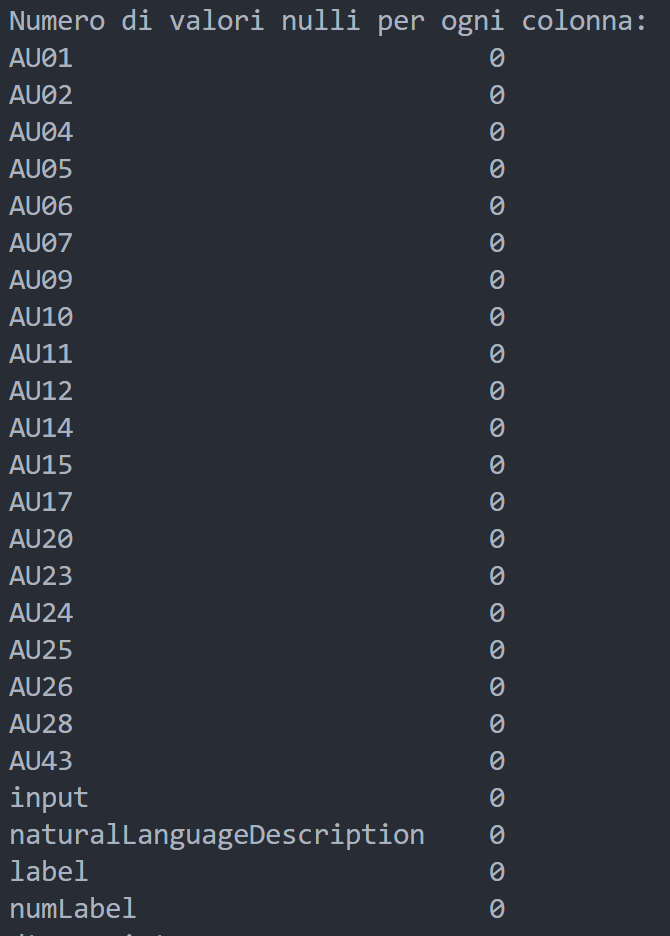
\includegraphics[width=0.4\linewidth]{images/image35.png}
            \end{center}
        \end{figure}
        Come è possibile osservare dall’immagine, il dataset risultato non presenta valori nulli.
    \end{itemize}
    \item aggiunta del valore di frame per ognuna delle analisi dei video:
    \begin{itemize}
        \item ogni analisi dei singoli frame di un video presentava lo stesso percorso di input (il file video associato); di conseguenza ho aggiunto alla fine del valore della colonna di input il frame dal quale sono state estratte le analisi.
    \end{itemize}
    \item rimozione delle colonne che non riguardano le Action Units
    \item aggiunta colonne al dataset
    \begin{itemize}
        \item label:
        \begin{itemize}
            \item le analisi inizialmente estrapolate non presentavano già le relative label; è stato quindi opportuno aggiungere.
        \end{itemize}
        \item numLabel
        \begin{itemize}
            \item ho associato ad ognuna delle label presenti un numero da 0 a 5:
            \begin{itemize}
                \item 0 $\rightarrow$ confused
                \item 1 $\rightarrow$ engaged
                \item 2 $\rightarrow$ frustrated
                \item 3 $\rightarrow$ bored
                \item 4 $\rightarrow$ drowsy
                \item 5 $\rightarrow$ looking away
            \end{itemize}
        \end{itemize}
        \item descrizione in linguaggio naturale descritta precedentemente
    \end{itemize}
\end{itemize}

\section{Resampling del dataset per migliorare la precisione delle predizioni} 
Il dataset risultato da me realizzato presenta una notevole complicazione: se decidessi di effettuare delle predizioni attraverso uno dei classificatori generati direttamente dal dataset as-his, il numero di campioni (samples) per ognuno dei valori della colonna labels risulterebbe sbilanciato.

Per sbilanciato intendo il fatto che sono presenti molti valori per alcune delle classi (labels), e troppi pochi, a confronto, per altri.
\begin{figure}
    \begin{center}    
        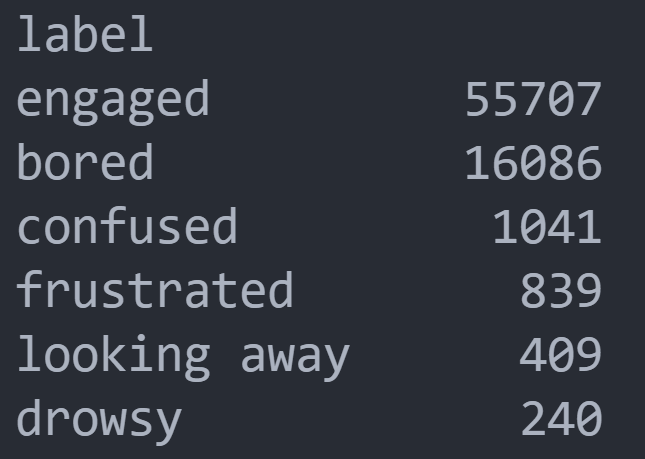
\includegraphics[width=0.4\linewidth]{images/image42.png}
    \end{center}
\end{figure}

In questi grafici è possibile riscontrare la differenza fra il numero di elementi per ogni valore unico nella colonna label:
\begin{figure}
    \begin{center}    
        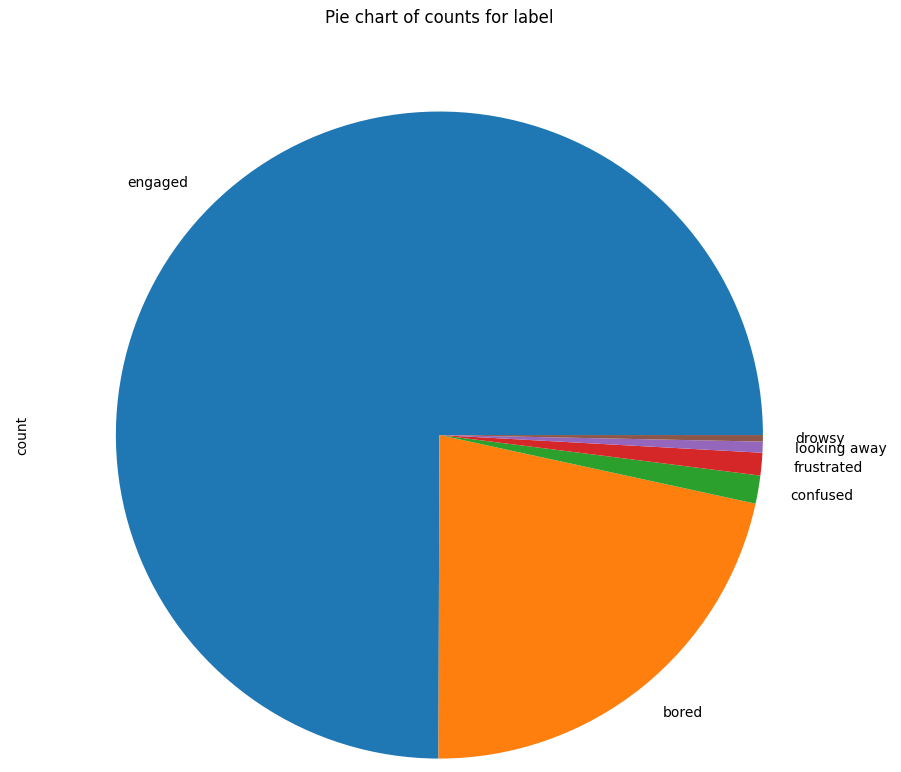
\includegraphics[width=0.8\linewidth]{images/image43.png}
    \end{center}
\end{figure}
\begin{figure}
    \begin{center}    
        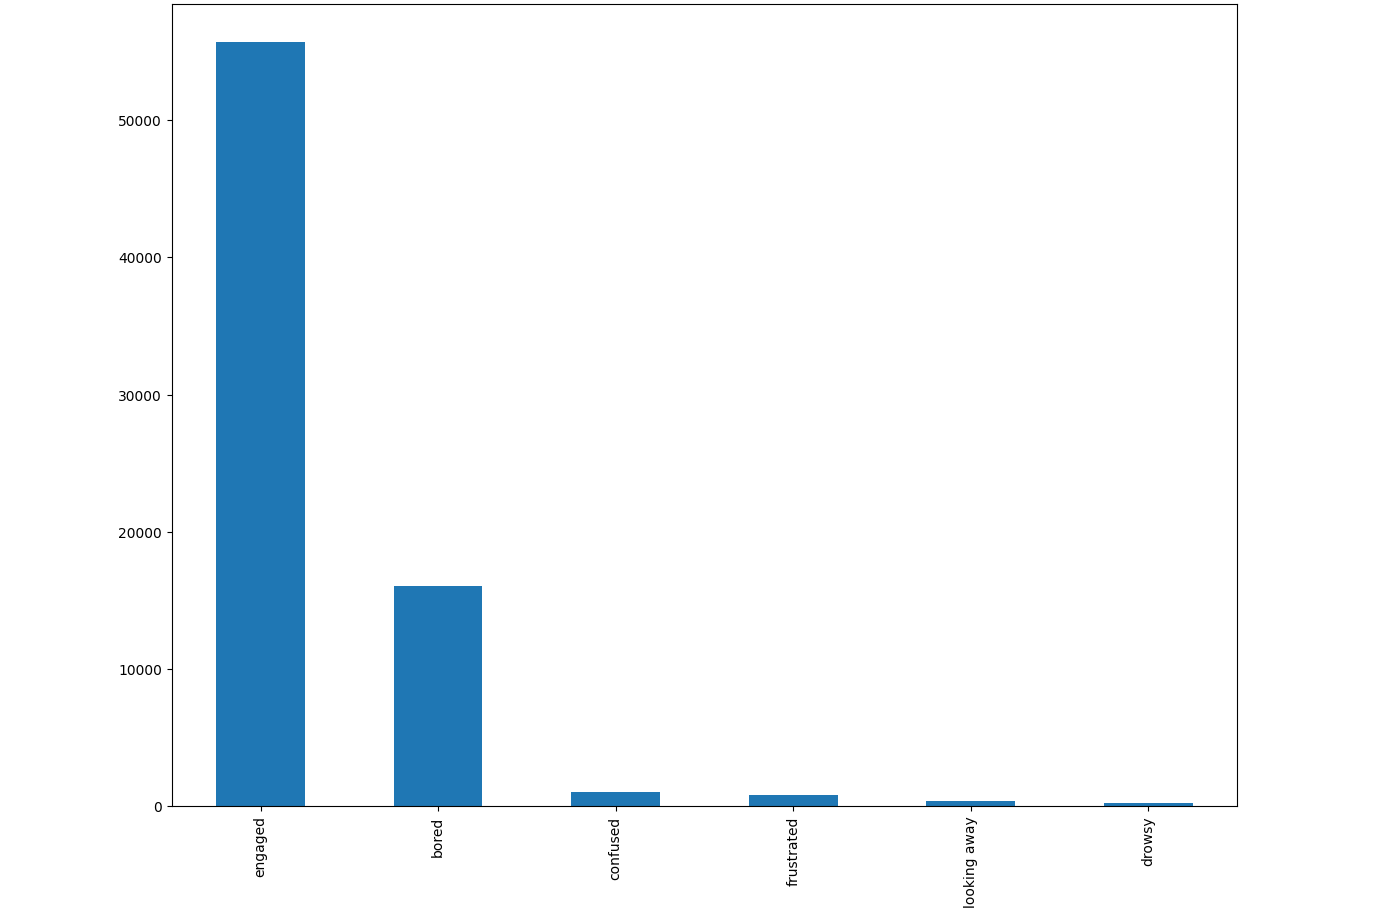
\includegraphics[width=0.8\linewidth]{images/image44.png}
    \end{center}
\end{figure}

Il resampling, che prevede una modifica  della distribuzione dei dati di un dataset mediante la rimozione o l’aggiunta, in modo casuale, di valori simili a quelli delle sue istanze, è una tecnica comune per bilanciare dataset sbilanciati o per migliorare le prestazioni di modelli di machine learning. Esistono due tipi principali di resampling: undersampling e oversampling:
\begin{itemize}
    \item L'undersampling, come suggerisce il nome, consiste nel rimuovere alcune delle istanze della classe maggioritaria (ovvero quella con un maggior numero di campioni) in modo da bilanciare la distribuzione delle classi nel dataset. 
    
Ciò può essere effettuato in modo casuale, pur essendo possibile utilizzare tecniche più sofisticate, come l'eliminazione degli esempi più vicini (nearest neighbor deletion) o la selezione degli esempi più rappresentativi (prototype selection). 

Il codice utilizzato per effettuare l’undersampling dei sample per ognuna delle labels è il seguente:
\begin{minted}[bgcolor=bg, fontsize=\scriptsize]{python}
def undersampleDataset(df, columnName, valueToDownSample, numberOfSamplesAfter):
    if len(df[df[columnName] == valueToDownSample]) > numberOfSamplesAfter:
        engagedIndices = df[df[columnName] == valueToDownSample].index
        tempDf = df.loc[engagedIndices]
        tempDfUndersampled = tempDf.sample(n=numberOfSamplesAfter, random_state=69)
        return pd.concat([df.drop(engagedIndices), tempDfUndersampled])
    return df
\end{minted}
\item L'oversampling, d'altra parte, consiste nell'aumentare il numero di istanze della classe minoritaria (ovvero quella con un minor numero di campioni) in modo da bilanciare la distribuzione delle classi nel dataset.

Sussistono molte tecniche per l'oversampling, tra cui la duplicazione casuale degli esempi esistenti, la generazione di nuovi esempi sintetici attraverso tecniche come la Synthetic Minority Over-sampling Technique (SMOTE), e la duplicazione degli esempi esistenti con una variazione minore (data augmentation). 
Il codice utilizzato per effettuare l’oversampling dei sample per ognuna delle labels è il seguente:
\begin{minted}[bgcolor=bg, fontsize=\scriptsize]{python}
def oversampleDataset(df, columnName, valueToOversample, numberOfSamplesAfter):
    if len(df[df[columnName] == valueToOversample]) < numberOfSamplesAfter:
        engagedIndices = df[df[columnName] == valueToOversample].index
        
        tempDf = df.loc[engagedIndices]
        tempDfOversampled = resample(
            tempDf, 
            replace=True, 
            n_samples=numberOfSamplesAfter, 
            random_state=69
        )
        
        return pd.concat([df.drop(engagedIndices), tempDfOversampled])
    return df
\end{minted}

\end{itemize}

In sintesi, il resampling è una tecnica utile per bilanciare dataset e migliorare le prestazioni dei modelli di machine learning. 

Questo invece è il codice che gestisce le chiamate per entrambi i metodi riportati sopra:
\begin{minted}[bgcolor=bg]{python}
def resampleDataset ():
    df = pd.read_csv(oldDatasetPath)
    visualizeDataFrameChart(df)

    numberOfValuesForEachLabel = 2000

    labelsList = df["label"].unique()
    for label in labelsList:
        df = undersampleDataset (
            df, 
            "label", 
            label, 
            numberOfValuesForEachLabel
        )
    for label in labelsList:
        df = oversampleDataset (
            df, 
            "label", 
            label, 
            numberOfValuesForEachLabel
        )

    visualizeDataFrameChart(df)

   df.to_csv(newDatasetPath, index=False)
\end{minted}

\begin{enumerate}
\item sklearn.utils.resample è una funzione fornita dalla libreria scikit-learn che viene utilizzata al fine di generare esempi sintetici per l'oversampling di dataset. In particolare, la funzione resample prende in input un insieme di campioni e genera un nuovo insieme di campioni sintetici.

La funzione resample prende in input i seguenti parametri:
\begin{itemize}
\item X: un array o un dataframe che rappresenta le feature dei campioni
\item y: (non valorizzato) un array o un dataframe che rappresenta le label dei campioni
\item replace: un valore booleano che indica se l'oversampling deve essere fatto con o senza sostituzione (ovvero se gli esempi sintetici possono essere duplicati)
\item n\_samples: il numero di esempi sintetici da generare
\item random\_state: un valore intero che rappresenta il seed per la generazione casuale degli esempi sintetici
\end{itemize}
La funzione resample restituisce due oggetti:
\begin{itemize}
\item X\_resampled: un array o un dataframe contenente le feature dei campioni originali e dei nuovi esempi sintetici generati (unico output utilizzato)
\item y\_resampled: un array o un dataframe contenente le label dei campioni originali e dei nuovi esempi sintetici generati
\end{itemize}
In sostanza, la funzione resample genera nuovi esempi sintetici aggiungendo variazioni minime ai campioni esistenti, in modo da produrre una distribuzione bilanciata delle classi nel dataset. 

Questi nuovi esempi sintetici vengono poi utilizzati insieme ai campioni esistenti per addestrare i modelli di machine learning.


\item pandas.DataFrame.sample è una funzione fornita dalla libreria pandas che viene utilizzata per estrarre casualmente un sottoinsieme di righe da un dataframe. 

In particolare, la funzione sample prende in input un dataframe e restituisce un nuovo dataframe contenente solo un sottoinsieme delle righe del dataframe originale.
\begin{itemize}
    \item n: il numero di righe da estrarre casualmente
    \item frac: (non valorizzato) la frazione di righe da estrarre casualmente (ad esempio, 0.5 per estrarre il 50% delle righe)
    \item replace: (non valorizzato) un valore booleano che puntualizza se le righe estratte devono essere selezionate con o senza sostituzione (ovvero se una stessa riga può essere selezionata più volte)
    \item weights: (non valorizzato) un array di pesi per ogni riga, utilizzato per selezionare le righe in modo ponderato
    \item random\_state: un valore intero che rappresenta il seed per la generazione casuale degli indici delle righe da selezionare
\end{itemize}
La funzione sample restituisce un nuovo dataframe contenente solo il sottoinsieme delle righe selezionate casualmente dal dataframe originale. 
Fondamentalmente, la funzione sample è utilizzata per ridurre la dimensione del dataframe originale, selezionando solo un sottoinsieme casuale delle righe.
Ciò può dimostrarsi utile per ridurre i tempi di calcolo durante l'addestramento dei modelli di machine learning, in particolare quando il dataset originale è molto ampio e non è necessario utilizzare tutte le righe per ottenere un buon modello.
\end{enumerate}

Per l’appunto, prima di effettuare il resampling del dataset, ho provato ad effettuare delle analisi su nuove immagini utilizzando un classificatore generato dal dataset as-his e i risultati si sono rivelati quelli aspettati, ovvero:

Quasi sempre veniva rilevato che la persona ripresa nell’immagine aveva delle Action Units che portavano alla predizione “engaged” e le altre volte veniva rilevato lo stato d’animo “bored”, ignorando del tutto gli altri valori presenti per la colonna label.

Dopo aver messo in pratica vari test, sono giunto alla conclusione di eseguire un resample al fine di ottenere 2000 istanze per ogni label, in quanto questo sembra il numero di sample in grado di far conseguire risultati più corenti nel tempo; i risultati relativi ottenuti sono riportati nell’ultimo capitolo. 

Di seguito riporto i grafici riguardanti il dataset presentati all’inizio, generati dopo aver effettuato il resampling:
\begin{figure}
    \begin{center}    
        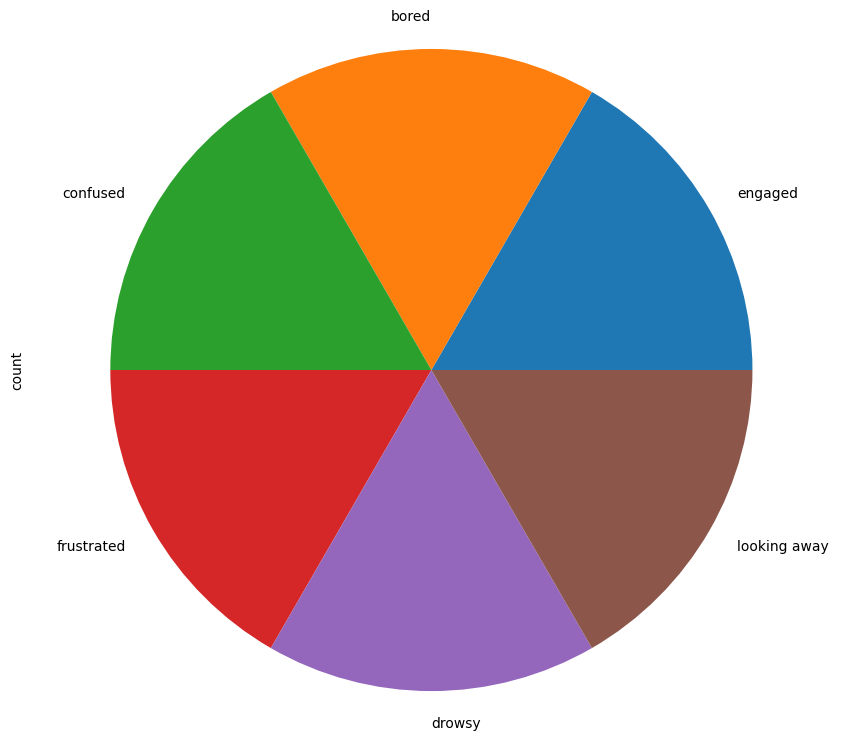
\includegraphics[width=0.9\linewidth]{images/image45.png}
    \end{center}
\end{figure}

\begin{figure}
    \begin{center}    
        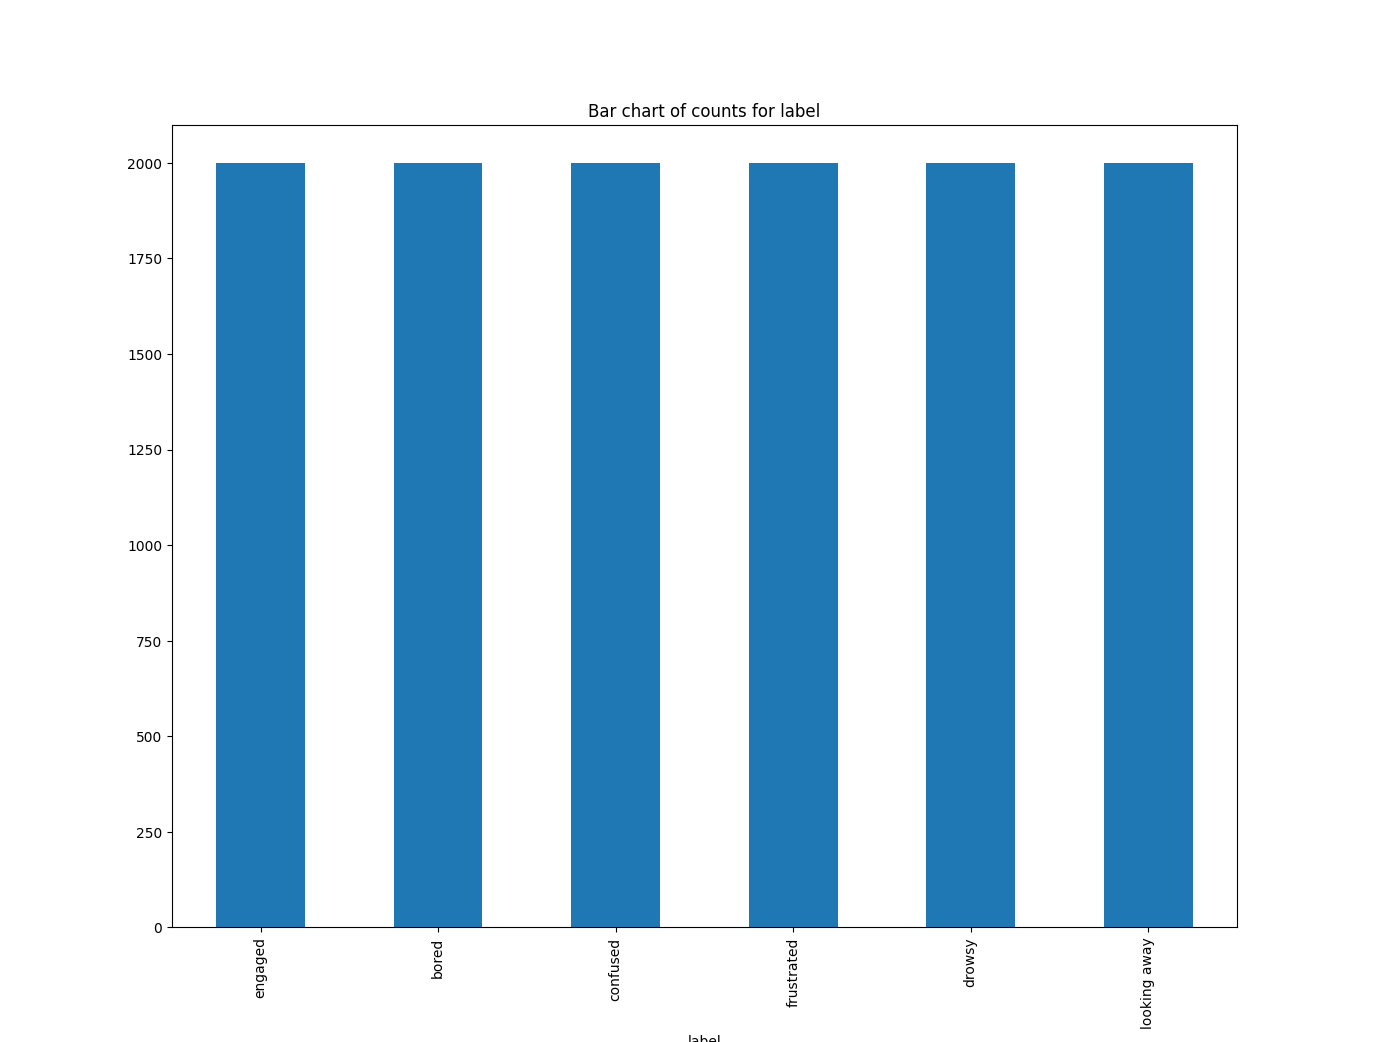
\includegraphics[width=0.9\linewidth]{images/image46.png}
    \end{center}
\end{figure}